\chapter{Methodology}
\label{ch:method}

\section{ESN Parameters and Sample Sizes}
\label{sec:esn-param}

In this section we present the baseline ESN used during experiments. For each
experiment described in this thesis, the default setup will be as described in
this section, unless otherwise specified. All ESNs are generated according to
the architecture presented in Figure \ref{fig:esn}.

We considered discrete-time ESNs with $N$ internal network nodes, a single
input, and a single output node. $\mathbf{W}^{in}$ was generated as a random
matrix with i.i.d. entries in the interval [-0.5, 0.5], and was fully
connected. In experiments with default ESNs, i.e. experiments where the internal
network $\mathbf{W}^{res}$ is not replaced, the weights were generated from the
same distribution as $\mathbf{W}^{in}$, but with a 10\% node connectivity. This
method for instantiating $\mathbf{W}^{res}$ and $\mathbf{W}^{in}$ is common
practice in RC \cite{montavon_practical_2012}.

In experiments where relevant, the reservoir weight matrix was rescaled such
that its spectral radius $\rho(\mathbf{W}^{res}) = 0.9$. The default input
scaling used was $\iota = 1.0$. Both parameters could be tuned to provide
marginally better results in most cases, but these values were found to give a
good baseline for comparisons between models.

$\mathbf{W}^{out}$ was adapted with ridge regression, using single value
decomposition for computational routines. This was found to lead to the most
stable and precise results.

% (TODO): Perhaps re-run everything with exactly 20 runs. We need the
% std. dev. anyway for tables in appendix.
For all experiment runs, the first 200 states of each run were discarded to
provide a washout of the initial reservoir state. Reported performances are the
mean across 20 randomizations of each model representative. This sample size was
found to be appropriate to pinpoint definite trends in the results. Standard
deviations for all experiments are thus provided in the appendix.

The Python software library implementation is available online, including a
Jupyter Notebook for reproducing each
experiment\footnote{\textcolor{red}{deadlink}}.

\section{Benchmarks and Metrics}
\label{sec:bench-metr}

\begin{figure}[t!]
  \centering
  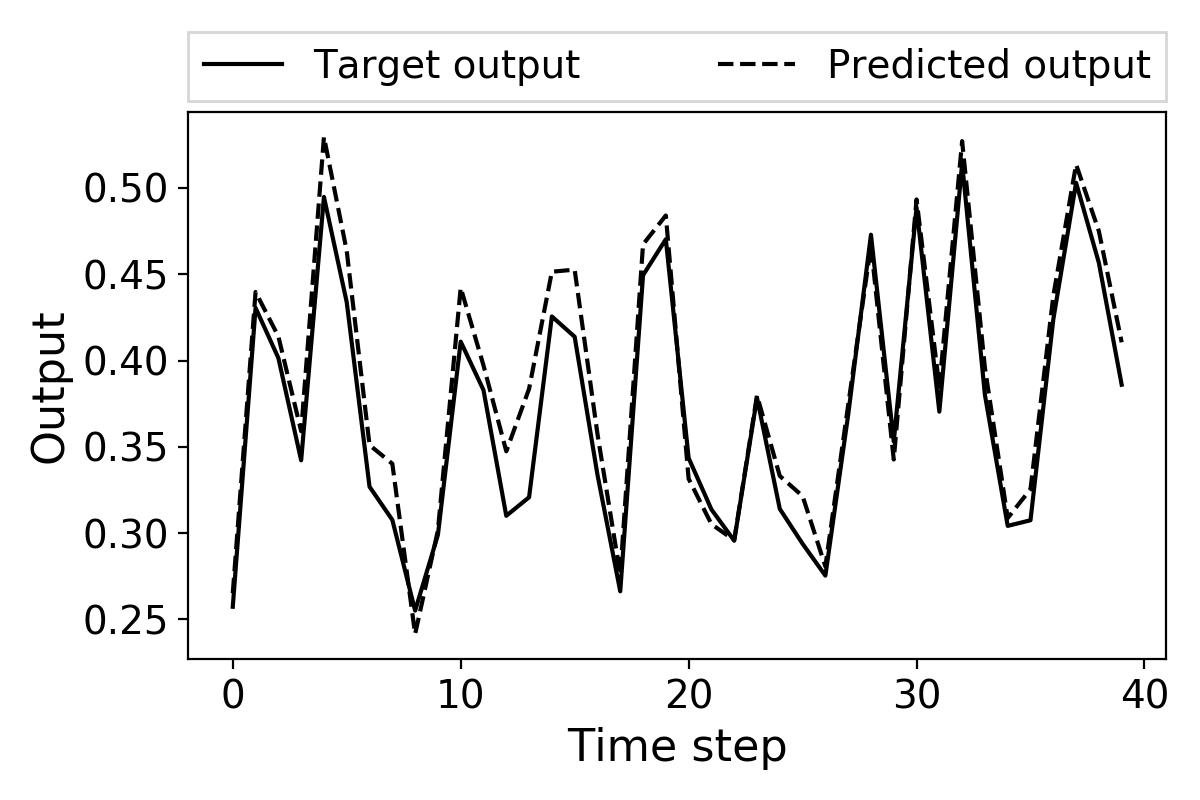
\includegraphics[width=3.0in]{figures/benchmark-example.png}
  \caption{
    Evaluation of a traditional ESN of size $N = 200$ on the NARMA-10
benchmark. The first 40 time steps of the benchmark are shown, comparing target
output to the predicted output of the reservoir. The resulting NRMSE was 0.23.
  }
  \label{fig:benchmark-example}
\end{figure}

To evaluate reservoirs, the benchmarks and metrics described in Section
\ref{sec:benchmark} were used. Note that the our primary evaluation tool was the
NARMA-10 benchmark, using the rest as supplements where relevant.

For the NARMA-10 benchmark, We generated the time series according to Equation
\ref{eq:narma}. The generated input was split into a training and test set, with
$L_{train} = 2000$ and $L_{test} = 3000$, to allow comparisons with results
presented in \cite{rodan_minimum_2011}.

The Mackey-Glass benchmark has been used in a range of ways, making comparison
of models harder than for NARMA. We used the method presented in
\cite{ma_deep-esn:_2017}. We generated a time series from Equation \ref{eq:mg17}
using discrete approximation, squashing the output into a range of [-1, 1] with
$\tanh(y-1)$. The series was split into a training and test set, with $L_{train}
= 6400$ and $L_{test} = 2000$. The task of the reservoir was to predict input 84
time steps ahead, i.e. $\mathbf{y}(t) = \mathbf{u}(t+84)$.

To evaluate performance on the benchmark, we used the normalized root mean
square error (NRMSE). The NRMSE is a commonly used error metric, providing
comparability to performances reported in previous work. Given a predicted
signal $\mathbf{y}(t)$ and a target signal $\mathbf{\hat{y}}(t)$

\begin{equation}
  \textrm{NRMSE}(\mathbf{y}, \mathbf{\hat{y}}) = \sqrt{\frac{
      \mean{\norm{\mathbf{y}(t) - \mathbf{\hat{y}}(t)}^{2}}
    }{
      \mean{\norm{\mathbf{\hat{y}}(t) - \mean{\mathbf{\hat{y}}(t)}}^{2}}
    }
  }
  .
  \label{eq:nrmse}
\end{equation}

An evaluation of a traditional ESN of size $N = 200$ using the NARMA-10
benchmark is shown in Figure \ref{fig:benchmark-example}. In this figure, the
first 40 time steps of the benchmark are shown, comparing the target output to
the predicted output of the reservoir. The resulting NRMSE of the benchmark was
0.23.

Kernel quality was evaluated by drawing $N$ input streams of length 20 uniformly
from the interval [-1, 1], where $N$ is the number of hidden nodes. The
resulting input streams were then run through the reservoir, and the rank of the
resulting $N \times N$ matrix, consisting of the reservoir states, was
computed. Generalization ability was evaluated in a similar manner, but
differing in that the last four inputs across all input streams were
identical. This is a standard way of computing the metrics
\cite{busing_connectivity_2010}.

Memory capacity was computed according to \cite{farkas_computational_2016}. An
input stream of length 2200 was drawn uniformly from the interval [-1, 1], and
the first 200 inputs were discarded to get rid of transients. Next, an input
sequence of length 1000 was used for training, and the remaining 1000 inputs for
testing. Memory capacity was computed according to Equation \ref{stm-eq}, using
$k = 1.4N$ output neurons.

\section{Experiments}

In chapter \ref{ch:rgg} we are concerned with replacing the generated
$\mathbf{W}^{res}$ with one that is generated as a random geometric graph. In
chapter \ref{ch:regular-tilings} we replace the matrix with reservoirs in which
the internal connectivity is set to be square, hexagonal and triangular regular
tilings. Beyond this, the ESN approach remains entirely the same, unless
explicitly stated otherwise.

%%% Local Variables:
%%% mode: latex
%%% TeX-master: "../thesis"
%%% End: